\documentclass[titlepage,landscape]{seminar}
\usepackage{url}
\usepackage{graphicx}
\usepackage{hyperref}
\usepackage{epstopdf}
\usepackage{slides}

\newcommand{\frack}{\frac{1}{k}}

\begin{document}

\myslide{
\heading{Principal components analysis of genotypes}

Principal components analysis is a ``dimension reduction'' method, a
way of reducing a very large number of variables to a smaller, more
manageable number for interpretation and analysis.

\begin{center}
  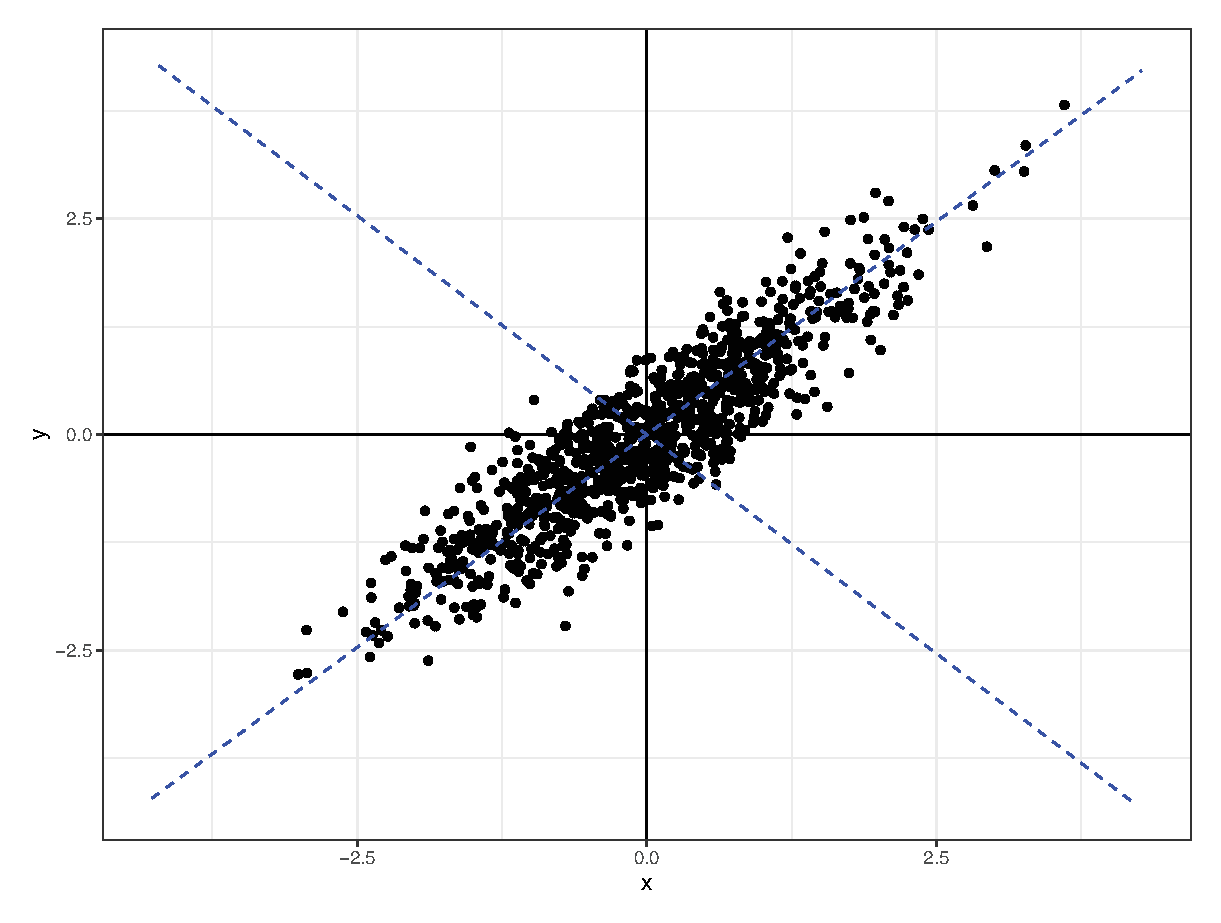
\includegraphics[height=5cm]{pca-example.eps}
\end{center}

\vfill\eject
}

\myslide{
\heading{Principal components analysis of genotypes}

3129 Europeans, 500,568 SNP loci

\begin{figure}
\begin{center}
\resizebox{0.5\textwidth}{!}{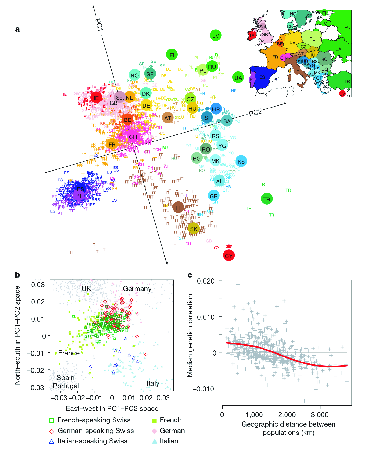
\includegraphics{human-PCA.eps}}
\end{center}
\end{figure}

\vfil\eject
}

\myslide{
\heading{Components of selection}

\begin{description}

\item[Assumption \#3:] {\it Meiosis is fair}.

\begin{itemize}

\item Segregation distortion

\item Gamete competition

\end{itemize}

\item[Assumption \#6:] {\it All matings produce the same number of
    progeny}.

\begin{itemize}

\item Fertility selection

\end{itemize}

\item[Assumption \#8:] {\it Survival does not depend on genotype}.

\begin{itemize}

\item Viability selection

\end{itemize}

\item[Assumption \#2:] {\it Individuals mate at random}.

\begin{itemize}

\item Sexual selection

\item Disassortative mating

\end{itemize}

\end{description}
}

\myslide{
\heading{Genetics of viability selection}
{\footnotesize
\begin{center}
\begin{tabular}{cc}
\hline\hline
Symbol  & Definition \\
\hline
$N$      & number of individuals in the population \\
$x_{11}$ & frequency of $ST/ST$ genotype \\
$x_{12}$ & frequency of $ST/CH$ genotype \\
$x_{22}$ & frequency of $CH/CH$ genotype \\
$w_{11}$ & fitness of $ST/ST$ genotype, probability of surviving from
           egg to adult \\
$w_{12}$ & fitness of $ST/CH$ genotype \\
$w_{22}$ & fitness of $CH/CH$ genotype \\
\hline
\end{tabular}
\end{center}
}
}

\myslide{
\heading{Genetics of viability selection}
\begin{center}
\begin{tabular}{l|ccc}
\hline\hline
Genotype         & $ST/ST$    & $ST/CH$    & $CH/CH$    \\
\hline
Number in eggs   & 41       & 82       & 27       \\
viability        & 0.6      & 0.9      & 0.45     \\
Number in adults & 25       & 74       & 12       \\
\hline
\end{tabular}
\end{center}
\begin{eqnarray*}
p\mbox{ ``before selection''} &=& (2\times 41 + 82)/(2\times 41 +
                                  2\times 82 + 2\times 27) \\
                              &=& 0.55 \\
p\mbox{ ``after selection''} &=& (2\times 25 + 74)/(2\times 25 +
                                  2\times 74 + 2\times 12) \\
                             &=& 0.56
\end{eqnarray*}
}

\myslide{
\heading{Genetics of viability selection}
\begin{center}
\begin{tabular}{l|ccc}
\hline\hline
Genotype         & $ST/ST$    & $ST/CH$    & $CH/CH$    \\
\hline
Number in eggs   & 41       & 82       & 27       \\
                 & $x_{11}N$  & $x_{12}N$  & $x_{22}N$  \\
viability        & 0.6      & 0.9      & 0.45     \\
                 & $w_{11}$   & $w_{12}$   & $w_{22}$   \\
Number in adults & 25       & 74       & 12       \\
                 & $w_{11}x_{11}N$ & $w_{12}x_{12}N$ & $w_{22}x_{22}N$ \\
\hline
\end{tabular}
\end{center}
}

\myslide{
\heading{Genotype frequencies}
\begin{eqnarray*}
\mbox{freq($ST/ST$) before selection}
 &=& \frac{41}{41 + 82 + 27} \\
 &=& 0.27 \\
\mbox{freq($ST/ST$) before selection}
 &=& \frac{Nx_{11}}{Nx_{11} + Nx_{12} + Nx_{22}} \\
 &=& x_{11} \\
 && \\
\mbox{freq($ST/ST$) after selection}
 &=& \frac{25}{25 + 74 +12} \\
 &=& 0.23 \\
\mbox{freq($ST/ST$) after selection}
 &=& \frac{w_{11}x_{11}N}{w_{11}x_{11}N + w_{12}x_{12}N + w_{22}x_{22}N} \\
 &=& \frac{w_{11}x_{11}}{w_{11}x_{11} + w_{12}x_{12} +
 w_{22}x_{22}} \\
 &=& \frac{w_{11}x_{11}}{\bar w}
\end{eqnarray*}
}

\myslide{
\heading{Mean fitness}
\begin{eqnarray*}
 \bar w &=& \frac{w_{11}x_{11}N + w_{12}x_{12}N + w_{22}x_{22}N}{N} \\
        &=& w_{11}x_{11} + w_{12}x_{12} + w_{22}x_{22} \quad .
\end{eqnarray*}
}

\myslide{
\heading{Allele frequencies}
\begin{eqnarray*}
\hbox{freq($ST$) before selection}
 &=& \frac{2(41) + 82}{2(41 + 82 + 27)} \\
 &=& 0.55 \\
\hbox{freq($ST$) before selection}
 &=& \frac{2(Nx_{11}) + Nx_{12}}{2(Nx_{11} + Nx_{12} + Nx_{22})} \\
 &=& x_{11} + x_{12}/2 \\
&& \\
\hbox{freq($ST$) after selection}
 &=& \frac{2(25) + 74}{2(25 + 74 + 12)} \\
 &=& 0.56 \\
\hbox{freq($ST$) after selection}
 &=& \frac{2w_{11}x_{11}N + w_{12}x_{12}N}{2(w_{11}x_{11}N + w_{12}x_{12}N + w_{22}x_{22}N)} \\
 &=& \frac{2w_{11}x_{11} + w_{12}x_{12}}{2(w_{11}x_{11} + w_{12}x_{12}
     + w_{22}x_{22})}
\end{eqnarray*}
}

\myslide{
\heading{Allele frequencies}
\begin{eqnarray*}
p' &=& \frac{w_{11}x_{11} + w_{12}x_{12}/2}{w_{11}x_{11} +
 w_{12}x_{12} + w_{22}x_{22}} \\
x_{11} &=& p^2, \quad x_{12} = 2pq, \quad x_{22} = q^2 \\
p' &=& \frac{w_{11}p^2 + w_{12}pq}{w_{11}p^2 + w_{12}2pq + w_{22}q^2} \\
\bar w &=& w_{11}x_{11} + w_{12}x_{12} + w_{22}x_{22} \\
       &=& p^2w_{11} + 2pqw_{12} + q^2w_{22}
\end{eqnarray*}
}

\myslide{
\heading{Fisher's Fundamental Theorem of Natural Selection}

\[
\bar w' \ge \bar w \quad .
\]

}

\myslide{
\heading{Patterns of natural selection}
\begin{center}
\begin{tabular}{cc}
\hline\hline
Pattern & Description \\
\hline
Directional & $w_{11} > w_{12} > w_{22}$ \\
            & or \\
            & $w_{11} < w_{12} < w_{22}$ \\
Disruptive  & $w_{11} > w_{12}$, $w_{22} > w_{12}$ \\
Stabiliizing& $w_{11} < w_{12}$, $w_{22} < w_{12}$ \\
\hline
\end{tabular}
\end{center}
}

\myslide{
  \heading{Relative viabilities}

\[
  p' = \frac{w_{11}p^2 + w_{12}pq}{\bar w}
\]
\[
  p' = \frac{p^2 + (w_{12}/w_{11})pq}{(\bar w/w_{11})}
\]

\begin{center}
\begin{tabular}{c|ccc}
\hline\hline
         & \multicolumn{3}{c}{Fitnesses} \\
 & $A_1A_1$ & $A_1A_2$ & $A_2A_2$ \\
\hline
First line & $w_{11}$ & $w_{12}$ & $w_{22}$ \\
Second line & 1 & $w_{12}/w_{11}$ & $w_{22}/w_{11}$ \\
\hline
\end{tabular}
\end{center}

\vfill\eject
}

\myslide{
\heading{Marginal fitnesses}
\begin{eqnarray*}
\Delta p &=& p' - p \\
&=& \frac{w_{11}p^2 + w_{12}pq}{\bar w} - p \\
&=& \frac{w_{11}p^2 + w_{12}pq - \bar wp}{\bar w} \\
&=& \frac{p(w_{11}p + w_{12}q - \bar w)}{\bar w} \\
&=& \frac{p(w_1 - \bar w)}{\bar w} \quad ,
\end{eqnarray*}
}

\myslide{
  \heading{Fertility selection}

\begin{center}
\begin{tabular}{c|ccc}
\hline\hline
                  & \multicolumn{3}{c}{Paternal genotype} \\
Maternal genotype & $A_1A_1$ & $A_1A_2$ & $A_2A_2$ \\
\hline
$A_1A_1$ & $F_{11,11}$ & $F_{11,12}$ & $F_{11,22}$ \\
$A_1A_2$ & $F_{12,11}$ & $F_{12,12}$ & $F_{12,22}$ \\
$A_2A_2$ & $F_{22,11}$ & $F_{22,12}$ & $F_{22,22}$ \\
\hline
\end{tabular}
\end{center}

$$
x_{11}' = \frac{x_{11}^2F_{11,11} + x_{11}x_{12}(F_{11,12} +
                F_{12,11})/2 + (x_{12}^2/4)F_{12,12}}{\bar F} \quad ,
$$
}

\myslide{
  \heading{Fertility selection}

  $\bar F'$ may {\it decrease} from one generation to the next.

  High fertility of heterozygote $\times$ heterozygote matings doesn't
  guarantee polymorphism.

  Selection may prevent loss of either allele, but there may not be a
  stable equilibrium.
}

\myslide{
\heading{Estimating fitnesses}
\begin{center}
\begin{tabular}{l|ccc}
\hline\hline
Genotype & $A_1A_1$ & $A_1A_2$ & $A_2A_2$ \\
\hline
Number in zygotes & $n_{11}^{(z)}$ & $n_{12}^{(z)}$ & $n_{22}^{(z)}$ \\
Viability         & $w_{11}$ & $w_{12}$ & $w_{22}$ \\
Number in adults  & $n_{11}^{(a)} = w_{11}n_{11}^{(z)}$ & $n_{12}^{(a)} = w_{12}n_{12}^{(z)}$ & $n_{22}^{(a)} = w_{22}n_{22}^{(z)}$ \\
\hline
\end{tabular}
\end{center}
}

\myslide{
\heading{Estimating fitnesses}
\begin{center}
\begin{tabular}{l|ccc}
\hline\hline
Genotype & $A_1A_1$ & $A_1A_2$ & $A_2A_2$ \\
\hline
Frequency in zygotes & $x_{11}^{(z)}$ & $x_{12}^{(z)}$ &
$x_{22}^{(z)}$ \\
Frequency in adults  & $x_{11}^{(a)}$ & $x_{12}^{(a)}$ &
$x_{22}^{(a)}$ \\
\hline
\end{tabular}
\end{center}
\vfill
\begin{eqnarray*}
x_{11}^{(a)} &=& w_{11}x_{11}^{(z)}/\bar w \\
x_{12}^{(a)} &=& w_{12}x_{12}^{(z)}/\bar w \\
x_{22}^{(a)} &=& w_{22}x_{22}^{(z)}/\bar w 
\end{eqnarray*}
\vfill
\begin{eqnarray*}
x_{11}^{(a)}/x_{12}^{(a)} &=& w_{11}x_{11}^{(z)}/w_{12}x_{12}^{(z)} \\
1 &=& 1 \\
x_{22}^{(a)}/x_{12}^{(a)} &=& w_{22}x_{22}^{(z)}/w_{12}x_{12}^{(z)}
\end{eqnarray*}
}

\myslide{
\heading{Estimating fitnesses}
\begin{eqnarray*}
\frac{w_{11}}{w_{12}} &=& \left(\frac{x_{11}^{(a)}}{x_{12}^{(a)}}\right)
                          \left(\frac{x_{12}^{(z)}}{x_{11}^{(z)}}\right) \\
\frac{w_{22}}{w_{12}} &=& \left(\frac{x_{22}^{(a)}}{x_{12}^{(a)}}\right)
                          \left(\frac{x_{12}^{(z)}}{x_{22}^{(z)}}\right)
\end{eqnarray*}
}

\myslide{
\heading{Estimating fitnesses}
\begin{center}
\begin{tabular}{l|ccc|c}
\hline\hline
Genotype & $ST/ST$ & $ST/CH$ & $CH/CH$ & Total \\
\hline
Number in larvae & 41 & 82 & 27 & 150 \\
Number in adults & 57 & 169 & 29 & 255 \\
\hline
\end{tabular}
\end{center}
\vfill
\begin{eqnarray*}
\frac{w_{11}}{w_{12}} &=& \left(\frac{x_{11}^{(a)}}{x_{12}^{(a)}}\right)
                          \left(\frac{x_{12}^{(z)}}{x_{11}^{(z)}}\right)
= \left(\frac{57/255}{169/255}\right)
  \left(\frac{82/150}{41/150}\right)
= 0.67 \\
\frac{w_{22}}{w_{12}} &=& \left(\frac{x_{22}^{(a)}}{x_{12}^{(a)}}\right)
                          \left(\frac{x_{12}^{(z)}}{x_{22}^{(z)}}\right)
= \left(\frac{29/255}{169/255}\right)
  \left(\frac{82/150}{27/150}\right)
= 0.52 \quad .
\end{eqnarray*}
}

\myslide{
\heading{Testing for viability selection}
\begin{center}
\begin{tabular}{l|ccc}
\hline\hline
Genotype & $ST/ST$ & $ST/CH$ & $CH/CH$ \\
\hline
Expected & $\left(\frac{41}{150}\right)255$ &
  $\left(\frac{82}{150}\right)255$ & $\left(\frac{27}{150}\right)255$ \\
         & 69.7    & 139.4   & 45.9 \\
Observed & 57      & 169     & 29 \\
\hline
\multicolumn{4}{l}{$\chi^2_2 = 14.82$, $P < 0.001$}
\end{tabular}
\end{center}
\vfill
\begin{eqnarray*}
\frac{w_{11}}{w_{12}} &=& 1 - s_1 \\
\frac{w_{22}}{w_{12}} &=& 1 - s_2 \quad .
\end{eqnarray*}
}

\myslide{
\heading{Fertility selection}
\begin{center}
\begin{tabular}{c|ccc}
\hline\hline
                  & \multicolumn{3}{c}{Paternal genotype} \\
Maternal genotype & $A_1A_1$ & $A_1A_2$ & $A_2A_2$ \\
\hline
$A_1A_1$ & $F_{11,11}$ & $F_{11,12}$ & $F_{11,22}$ \\
$A_1A_2$ & $F_{12,11}$ & $F_{12,12}$ & $F_{12,22}$ \\
$A_2A_2$ & $F_{22,11}$ & $F_{22,12}$ & $F_{22,22}$ \\
\hline
\end{tabular}
\end{center}
\vfill
\begin{equation}
x_{11}' = \frac{x_{11}^2F_{11,11} + x_{11}x_{12}(F_{11,12} +
                F_{12,11})/2 + (x_{12}^2/4)F_{12,12}}{\bar F} \quad ,
\label{eq:fertility}
\end{equation}
}

\myslide{
\heading{Properties of fertility selection}
\begin{enumerate}

\item $\bar F'$ may be smaller than $\bar F$. Unlike selection on
viabilities in which fitness evolved to the maximum possible value,
there are situations in which fitness will evolve to the {\it
minimum\/} possible value when there's selection on
fertilities.\footnote{Fortunately, it takes rather weird fertility
schemes to produce such a result.}

\item A high fertility of heterozygote $\times$ heterozygote matings
is not sufficient to guarantee that the population will remain
polymorphic.

\item Selection may prevent loss of either allele, but there may be no
stable equilibria.

\end{enumerate}
}

\myslide{
\heading{Fertility selection: mating table}
\begin{center}
\begin{tabular}{rcccc}
                       &           & \multicolumn{3}{c}{Offsrping genotype} \\
Mating                 & Frequency     & $A_1A_1$ & $A_1A_2$ & $A_2A_2$ \\
\hline
$A_1A_1 \times A_1A_1$ & $x_{11}^fx_{11}^m$     &        1 &        0 &        0 \\
              $A_1A_2$ & $x_{11}^fx_{12}^m$ &    $\half$ &    $\half$ &        0 \\
              $A_2A_2$ & $x_{11}^fx_{22}^m$ &        0 &        1 &        0 \\
$A_1A_2 \times A_1A_1$ & $x_{12}^fx_{11}^m$ &    $\half$ &    $\half$ &        0 \\
              $A_1A_2$ & $x_{12}^fx_{12}^m$     &  $\fourth$ &    $\half$ &  $\fourth$ \\
              $A_1A_2$ & $x_{12}^fx_{22}^m$ &        0 &    $\half$ &    $\half$ \\
$A_2A_2 \times A_1A_1$ & $x_{22}^fx_{11}^m$ &        0 &        1 &        0 \\
              $A_1A_2$ & $x_{22}^fx_{12}^m$ &        0 &    $\half$ &    $\half$ \\
              $A_2A_2$ & $x_{22}^fx_{22}^m$     &        0 &
0 & 1 \\
\end{tabular}
\end{center}
}

\myslide{
\heading{Fertility selection and selection on one sex}
\begin{eqnarray*}
x_{11}^m &=& \frac{x_{11}a_{11}}{\bar a} \\
x_{12}^m &=& \frac{x_{12}a_{12}}{\bar a} \\
x_{22}^m &=& \frac{x_{22}a_{22}}{\bar a} \quad ,
\end{eqnarray*}
\vfill
\[
x_{11}' = \frac{x_{11}^2a_{11} + x_{11}x_{12}(a_{12} + a_{11})/2
                + x_{12}^2a_{12}/4}{\bar a} \label{eq:sexual}
\]
\vfill
\[
\begin{array}{cccc}
       & A_1A_1 & A_1A_2 & A_2A_2 \\
A_1A_1 & a_{11} & a_{12} & a_{22} \\
A_1A_2 & a_{11} & a_{12} & a_{22} \\
A_2A_2 & a_{11} & a_{12} & a_{22}
\end{array}
\]
}

\end{document}


